\chapter{Primera Iteración: Prototipo inicial}
\label{primeraiteracion}

\section{Arquitectura del Proyecto}
\label{it1arquitectura}
La arquitectura del proyecto está caracterizada por la dinamicidad y capacidad para adaptarse de sus clases. Permitiendo que tomen un rol u otro dependiendo de las clases que las definan. Es decir, una clase personaje debe adaptarse al rol de personaje que le toque interpretar, y al contexto que le pone dentro de la escena. Además, debe seleccionar el recurso que lo represente que cumpla con las condiciones que se den en ese momento dentro de la escena. Finalmente debe permitir la interactuación y ejecución de efectos que están asignados a si mismo.

En esencial, esto se puede explicar con el diagrama de clases muy simplificado de la figura 3. Este diagrama fue generado en esta iteración del proyecto, por lo que su formato es muy diferente al resto de diagramas que se muestran en posteriores iteraciones.

\begin{figure}[htb]
	\centerline{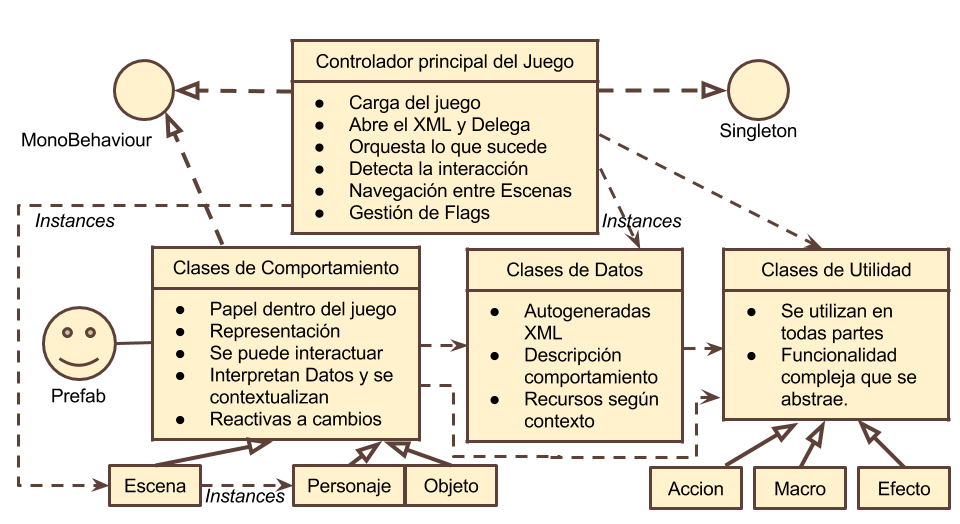
\includegraphics[height=3.5in]{figures/arquitecturait1.png}}
	\caption[Arquitectura simplificada - Prototipo 1]{Diagrama de clases simplificado de la arquitectura de clases de la primera iteración del proyecto.}
	\label{arquitecturait1}
\end{figure}

En la figura \ref{arquitecturait1} hay varios elementos que no son comunes en un diagrama de clases. El primero de ellos es la "Cara sonriente" que aparece a la izquierda con el texto \textit{Prefab} debajo de el. Este \textit{Prefab} es un elemento en Unity3D que resume el concepto de Objeto Prefabricado, y que, contiene, una representación tridimensional, junto a todas las componentes y comportamientos que definen dicho objeto. Por otra parte la interfaz \textit{MonoBehabiour} no es una interfaz, sino una clase abstracta, y esta, provee a los elementos que la extienden de la habilidad de ser componentes para los objetos de la escena. Dicha clase contiene varios métodos como Start(), Awake() o Update() que permiten a estos comportamientos inicializarse, actuar, y en esencia, tener una fracción de tiempo para realizar acciones dentro de la escena de Unity3D.

En la figura \ref{arquitecturait1} encontramos cuatro tipos de clases:

\begin{itemize}
	\item El controlador principal del juego.
	\item Las Clases de Datos
	\item Las Clases de Comportamiento: Escenas, Personajes, Objetos, Salidas, etc...
	\item Las Clases de Utilidad: Acciones, Efectos, Macros, Secuencias, Diálogos, etc...
\end{itemize}

Todas las clases que se presentan en este primer prototipo han sufrido cambios muy grandes o totales tanto en su código, como en su funcionalidad. Algunas de ellas han desaparecido, surgiendo clases nuevas que realizan su funcionalidad, otras se han transformado completamente o han sido asumidas por otras, y finalmente, otras han surgido de la generalización y refactorización de código.

\subsection{Controlador Principal de Juego}

El controlador principal de juego, implementado con una clase de nombre Game, se encarga de, en primer lugar, comenzar la carga del juego, comenzando a explorar el XML y delegando en las Clases de Datos su propia interpretación, así como orquestar lo que sucede dentro del juego, detecta la interacción por parte del jugador y notifica a aquellos elementos cuando se interactúa con ellos, realiza la navegación entre escenas cuando es necesario, y controla el estado de los interruptores que controlan las condiciones para la contextualización de cada escena en su momento apropiado.


Implementa el patrón Singleton, pues sólo una instancia es necesaria para el control.

\subsection{Clases de Datos}

Las clases de datos se encargan de generarse a partir de un elemento del fichero XML y sirven de descripción para una Clase de Comportamiento para representarse y interactuar de la forma correcta en cada momento. A través del documento XML realizan una lectura del mismo mediante la librería de c\# System.Xml, y rellenan sus atributos a partir de la especificación en dicho XML. Asimismo implementan funciones útiles como la obtención de un paquete de recursos apropiado según el contexto.

Existe una clase de datos por cada Clase de Comportamiento, aunque también existen clases de datos auxiliares mucho más pequeñas y que apenas aportan funcionalidad, siento meros contenedores de datos.

\subsection{Clases de Comportamiento}

Las clases de comportamiento son aquellas clases que juegan un papel dentro del videojuego y participan de forma activa en la representación del mismo. Dentro de esta categoría encontramos a las Escenas, los Personajes, los Objetos, las Salidas de las escenas, así como los objetos de atrezo y todos aquellos elementos que tienen una representación virtual en el videojuego. 

Cada una de estas clases heredará de la clase de Unity \textit{MonoBehabiour}, que indica, como se explica en la sección \ref{it1arquitectura}, que dicha clase es un comportamiento y se puede asignar como componente a un elemento de la escena. Cada una de ellas tiene un objeto de datos que debe interpretar. Esta clase de comportamiento recibirá estímulos por parte del controlador principal del juego cuando el jugador interactue con ellas. Este paso intermedio es necesario ya que hay momentos en los que el controlado principal debe evitar la interacción del jugador con dichos elementos por encontrarse en mitad de un diálogo. Con este estímulo, la clase de comportamiento gestiona las diferentes interacciones que tenga el usuario con si mismo.

Finalmente, estas clases se encapsulan dentro de un \textit{Prefab}, formando parte como componente de un objeto tridimensional, junto a otras componentes.

\section{Detalles de la implementación}

Existen algunas cuestiones cruciales y generales acerca de cómo se realizó la implementación de diversas mecánicas que eran necesarias para que el juego funcionase.

Algunas de estas decisiones cruciales son, por ejemplo, la decisión de \textit{reRenderizar}\footnote{Renderizar es el proceso de generar una imagen, mediante el cálculo de la iluminación, a partir de un modelo 3D. En este caso se refiere a regenerar la representación de la escena.} la escena junto con todos sus elementos cada vez que un \textit{Flag}\footnote{Una Flag, bandera en Inglés, es un elemento que se utiliza para establecer hitos dentro del juego, como haber hablado con un personaje, o haber fallado una respuesta.} o una Variable de entorno cambia. Esto puede tener efectos devastadores si nuestra escena tiene elementos que han sido modificados por el jugador en un momento determinado, pero en el caso del videojuego Checklist, no existen dichos elementos, por lo que, cada vez que se activa un flag, en lugar de notificar a cada uno de los elementos, se \textit{renderiza} de nuevo la escena entera.

Esta decisión se tomó debido a que, pese a que existía la opción de implementar el patrón Observador-Observable, y hacer que todos los elementos de la escena fueran observadores y fuesen notificados cuando el estado del juego cambie, es frecuente que ocurra que, un elemento de la escena que en ese momento no tiene representación física, deba de reaccionar a este cambio en el estado del juego, y debido a que nunca recibirá la notificación, porque no existe, nunca aparecería.

No obstante esta decisión de volver a generar la escena, pese a que se mantiene, evolucionará en la siguiente iteración del proyecto, permitiendo al usuario modificar los elementos que se hallen dentro de la escena, guardando en un diccionario, referencias a los contextos dentro de las mismas. Por el momento no se han encontrado problemas de rendimiento con esta decisión, ya que las escenas, en general, suelen estar formadas por pocos elementos. Si se encontrasen dichos problemas, se desarrollaría un método más eficiente.

Otra de las decisiones cruciales de la implementación consistió en decidir si generar un \textit{SecuenceManager} que gestiona por completo las secuencias que se dan, como efectos, o diálogos; o por otra parte, hacer que las propias clases de \textit{GraphConversation} y \textit{Effect} fuesen capaces de ejecutarse por sí solas.

Después de comenzar con la implementación del \textit{SecuenceManager}, y construir una pila de secuencias, se vió que sería considerablemente complejo recordar datos contextuales acerca del estado de cada secuencia en caso de que fuese necesario parar la ejecución, y se decidió que era más sencillo que cada secuencia recordase por sí misma su posición.

En una sección posterior se detallan en profundidad los detalles de la implementación de las clases Conversation y Effect, dos clases que implementan la interfaz Secuence, y que permiten ser ejecutadas por si mismas.

\subsection{Sobre la clase Game}
\label{gameit1}

La clase Game es el Controlador principal del juego, y por ello realiza todas las funciones anteriormente descritas.

Sus funcionalidades se podrían categorizar en 4 apartados:

\begin{itemize}
	
	\item En primer lugar, y en la parte de más arriba del código se encuentra la gestión del \textit{singleton} y del acceso a las variables de entorno. Es decir, se facilita el acceso a las \textit{Flags} del juego, a las Variables, a la obtención de \textit{Macros}, Las especificaciones de los diálogos, etc. Esta parte es vital para el control del juego, y su estado.
	
	\item En segundo lugar, tras todas estas funciones, se encuentra el cargador de juego. Se ha implementado mediante el uso de un \textit{Thread}\footnote{Un Thread, en programación, es un proceso que se ejecuta de forma paralela a la ejecución del programa, por lo que permite la realización de múltiples tareas simultáneamente} que permite visualizar el estado de la carga del juego mientras esta se realiza, y, como Unity no permite cargar recursos con \textit{Resources.Load()} fuera del bucle principal del juego, se utiliza la librería del sistema \textit{System.IO.File} para leer directamente los ficheros y generar texturas con ellos. Aquí entra en juego la clase \textit{Texture2DHolder} de la que se realiza una explicación posteriormente.
	
	Este cargador prepara el fichero XML utilizando la librería del sistema System.Xml, y lo secciona en pequeños bucles, uno por cada elemento del juego, es decir, uno por personajes, otro por objetos, otro por escenas, etc. Cuando termina la carga, se cambia el estado de la clase \textit{Game} para comenzar con la visualización del juego.
	
	\item En tercer lugar, se encuentran determinadas funciones útiles que realizan tareas variadas como \textit{RenderScene}, para pintar una escena o \textit{Execute} para comenzar la ejecución de una secuencia, junto con la función \textit{Update()} donde se realiza parte del control del juego, junto con la gestión del click del usuario, donde bloquearemos dicho click, notificaremos al elemento clicado o simplemente extraemos las acciones disponibles de dicho elemento, dependiendo del estado del juego.
	
	\item Por último, y al final del código, se encuentra otra parte de interacción, junto con el pintado de la interfaz. Para la interfaz se ha generado una \textit{GUISkin}\footnote{Una GUISkin es un fichero de especificación de datos de Unity que contiene datos acerca de los elementos de la interfaz, como el tamaño de la fuente, colores de los fondos, o imágenes de los botones.} propia que se modifica en función del tamaño de la pantalla para hacerse más grande o pequeña dependiendo de su proporción. Para el pintado de la interfaz se ha utilizado \textit{GUILayout}, clase que facilita métodos para representar una interfaz, ya que se conocía su funcionamiento de haberla utilizado en proyectos anteriores, y era sencillo de implementar.
	
	Esta GUI, además de adaptarse, se ha preparado para que se posicione correctamente utilizando \textit{Camera.current.WorldToScreenPoint()}, es decir, que transforma los puntos del mundo tridimensional, a unas coordenadas de cámara, y mediante una serie de transformaciones, se colocan los cuadros en su lugar, evitando que estos cuadros de diálogo se salgan de la pantalla cuando un personaje habla desde uno de los extremos.
\end{itemize}

Esta explicación cierra, por encima, todos los elementos importantes de la implementación de la clase Game. Debido a que esta implementación no es la final, no se incluyen explicaciones más detalladas ni diagramas.

Esta clase es una de las clases que ha sufrido una mayor evolución en la segunda iteración, ya que, pese a que sigue controlando la interacción por parte del usuario, ya no realiza la lógica de dicha interacción en el bucle \textit{Update()}, sino que, simplemente delega en los diferentes elementos interactuados para que sean ellos los que realicen la lógica de su interacción. Asimismo, la gestión de la interfaz ha sido delegada en la clase \textit{GUIManager}, con un nuevo y rediseñado sistema de burbujas.

\subsection{Sobre las Clases de Datos}
\label{dataclassesit1}

Existen multitud de clases de datos dentro del código del programa, aunque todas se parecen bastante entre sí, por lo que se explicarán la mayoría de ellas en conjunto.

\begin{figure}[htb]
	\centerline{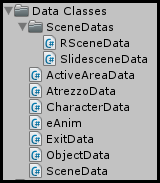
\includegraphics[height=2.5in]{figures/it1/dataclasses.png}}
	\caption[Clases de Datos - Prototipo 1]{Vista de carpeta de las clases de datos implementadas en la primera iteración.}
	\label{dataclassesfigit1}
\end{figure}

Estas clases se auto-generan analizando un \textit{XmlElement} que reciben en su constructor, y por lo general no aportan funcionalidad, salvo excepciones como la función \textit{Check()} que implementan la mayor parte de recursos para verificar si se cumplen todas las condiciones para que dicho recurso pueda ser utilizado.

La mayor parte de clases de datos contienen:
\begin{itemize}
	\item Una serie de Recursos: con soporte de videos y animaciones (implementadas con la clase eAnim y eFrame). Algunas clases implementan su propia clase para manejar sus recursos con Condiciones, como CharacterData con su CharacterResource, o SceneData con su SceneResource, aunque muchas otras simplemente utilizan diccionarios de tipo Dictionary<string,Texture2DHolder> Resources.
	
	\item También tienen una serie de condiciones ante las que decidiran representarese o no, estas condiciones son gestionadas mediante la clase Condition.
	
	\item Algunas clases de datos, además de Recursos y Condiciones, también tienen Efectos que se realizan al interactuar con ellas, o un listado de Acciones que se muestra como un menú contextual al interactuar con ellas.
\end{itemize}

Particularmente, existen algunas anomalías en las clases de datos, como son las clases que implementan la interfaz \textit{SceneData} la cual contiene, además de Recursos como todas las demás, gran variedad de objetos \textit{ItemReference}, los cuales contienen una referencia a un elemento de la escena (ya sea un personaje, objeto o una salida) y la contextualización del mismo, es decir, su posición en ese momento, las condiciones que tienen que darse para que ese elemento aparezca o no, etc.

La creación de dicha interfaz fué necesaria debido a que existen multitud de tipos de escenas. En este caso se han implementado 2 tipos de escenas que eran necesarias para el videojuego \textit{Checklist}, las \textit{RScene}, abreviando \textit{Regular Scene}, que son escenas normales sobre las que jugar, donde se representan personajes, objetos, salidas, áreas activas; y las \textit{Slidescene}, que son escenas con una sucesión de imágenes en su interior a modo de \textit{Slides} como si de una presentación se tratase.

Finalmente comentar que, algunas clases de datos como los \textit{ObjectData} o los \textit{ActiveAreaData} tienen un elemento llamado \textit{InfluenceArea} el cual no se ha implementado, y que permite que un objeto o un active área sea mucho más grande que su area de interacción, la cual está formada por una sucesión de puntos que generan al final un polígono. Esto permite que pueda haber un objeto con formas irregulares e interactuar con él sólo en las zonas de real contacto con la imagen. Por lo que todas nuestras áreas de influencia serán rectangulares.

Esta Área de Influencia, sin embargo, en la siguiente iteración del proyecto sí que ha sido implementada, mediante la utilización de librerías de triangulación de polígonos irregulares de cualquier tipo, y la transformación de dichos polígonos en Mallas tridimensionales. La explicación de dicha transformación será realizada en la siguiente iteración.

Finalmente, la clase eAnim tiene una peculiaridad, y es que en versiones antiguas de eAdventure, las animaciones se generaban a partir de secuencias de imágenes en la carpeta animations, carpeta utilizada para el almacenamiento de las imágenes que forman las animaciones.

Es decir, existen animaciones formadas de la siguiente manera: “anim\_01.png”, “anim\_02.png” y estas están especificadas en el fichero de especificación del juego de eAdventure como “/animaciones/anim”. Esto supone dos problemas. El primero consiste en identificar cuál es el formato del fichero de imagen, por lo que existe una lista de tipos disponibles y se intenta encontrar un archivo que satisfaga tanto el nombre de la animación, como el formato correspondiente. Y en segundo lugar, no se sabe cuántos archivos hay, lo que hace que debas iterar hasta que no encuentres fichero.

Por otra parte, el nuevo formato de animaciones está definido en ficheros XML llamados “.eaa” que son mucho más sencillos de recorrer y contienen más información acerca de cada fotograma de la animación.

\subsection{Sobre las Clases de Comportamiento}
\label{behavioursit1}

De manera similar al apartado anterior, se explicará el funcionamiento de la mayor parte de clases de comportamiento, puntualizando detalles acerca de algunas de dichas clases en concreto, como \textit{Character} o \textit{eObject}, que tienen comportamientos aislados como la gestión de fotogramas o la necesidad de cambiar cuando el usuario va a interactuar con ellos.

\begin{figure}[htb]
	\centerline{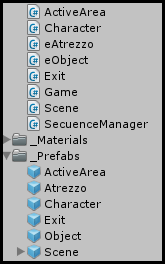
\includegraphics[height=3in]{figures/it1/behaviourclasses.png}}
	\caption[Clases de Comportamiento - Prototipo 1]{Vista de carpeta de las clases de comportamiento implementadas en la primera iteración, junto a sus Prefabs.}
	\label{behaviourclassesit1}
\end{figure}

Las clases de comportamiento son todas herederas de \textit{MonoBehabiour} por lo que se asignan a objetos dentro de la escena, y luego estos objetos se guardan en forma de \textit{Prefabs}, cada una a uno individualmente. Estos \textit{Prefabs} suelen ser muy sencillos, en su mayoría constituidos únicamente por un \textit{Quad}\footnote{Un Quad es una malla tridimensional compuesta por un plano, una de las mallas más simples.}, al cual se le cambia la textura con \textit{this.GetComponent<Renderer>().material.mainTexture}, y posteriormente, mediante la información de dicha textura, se aplican modificaciones escalando el Quad. 

Todas estas clases de comportamiento son la representación de algún elemento de la escena, y por ello tienen en su interior los siguientes elementos:

\begin{itemize}
	\item En primer lugar una clase de datos asignada que será el “Guión” de nuestra clase para enrolarse. Es decir: una clase \textit{Character} contendrá dentro una clase \textit{CharacterData}, o una clase \textit{eObject} (la letra e era necesaria porque la clase \textit{Object} ya existe en el espacio de nombres, y proviene de juntar eAdventure con \textit{Object}), contiene una clase \textit{ObjectData}.
	
	\item En segundo lugar, aunque no todas la tienen, una \textit{ItemReference}, que utilizan para contextualizarse. Un \textit{character} no sería capaz de conocer su posición dentro de la escena si no tuviera un \textit{ItemReference} para poder contextualizar, y tampoco sabría si ese es su momento de aparecer en la escena, o si no debe aparecer más.
	
	\item Por último contienen aquellas funciones que son necesarias para su correcto funcionamiento.
\end{itemize}

\subsubsection{Detalles de la clase Character}

La clase \textit{Character} contiene una serie de comportamientos necesarios y características específicas que hacen que sea diferente a las demás, pues tiene animación y ha de ir cambiando el fotograma que la representa con el paso del tiempo, por lo que en su función de comienzo de la ejecución, \textit{Start()}, selecciona la animación que cumple todas las condiciones, y establece el primer fotograma, y en su función de actualización del estado, \textit{Update()}, va cambiando su fotograma con la funcion \textit{ChangeFrame()}.

Esta función \textit{ChangeFrame()} accede al \textit{renderer}\footnote{El renderer, en Unity3D, es la componente de los objetos que tienen representación en la escena, que define cómo se representan en la misma, con características como los materiales que las conforman, las texturas, las mallas tridimensionales, y otros elementos.} y cambia su textura además de actualizar determinadas variables de control, que establecen cuando deberá realizarse el próximo cambio de fotograma, o el fotograma que se está representando actualmente.

\subsubsection{Detalles de la clase eObject, Exit y ActiveArea}
\label{objectexitactiveareait1}

Estas tres clases tienen la peculiaridad de que deben ser reactivas a interacción por parte del jugador, y mostrar algún cambio en su representación cada vez que el jugador pase el puntero del ratón por encima de ellas. Esto se implementó utilizando las funciones que facilita la clase \textit{MonoBehaviour}, I y \textit{OnMouseExit()} y que reciben el evento del puntero cuando este entra en su área de reacción y cuando sale de la misma.

Cada una de las tres clases que son reactivas a este evento realiza una acción diferente, donde, el \textit{eObject} cambia su imagen y, por otra parte, \textit{Exit} y \textit{ActiveArea}, acceden a su material para cambiar su color, volviéndose de color rojo la representación de \textit{Exit}, y de color verde la representación de una \textit{ActiveArea}.

Adicionalmente, la clase \textit{Exit} tiene una función \textit{exit()} que se encarga de ejecutar todos los efectos que conllevan la salida de la escena, así como de mandar el renderizado de la nueva escena.

Esta clase \textit{Exit}, en esta versión del intérprete, no funcionaba correctamente, pues una salida puede contener un \textit{not-effect}, es decir, un efecto que se debe de ejecutar si se intenta salir de la escena cuando las condiciones no lo permiten. Esto implica que, la salida debe de gestionar su propia representación, y la Escena debe delegar esta funcionalidad en la salida.

Por otra parte, y como ya se mencionó en un apartado anterior, las \textit{ActiveAreas} contienen una funcionalidad adicional en la última versión del intérprete, ya que estas se adaptan a un Área de Influencia, que modifica su contorno y forma, adaptándose a la forma de un polígono irregular definido por un listado de puntos en el fichero de especificación del juego.

\subsubsection{Detalles específicos de Scene}

La clase Scene supone un reto más complejo de abordar, en comparación con todas las demás clases de comportamiento, pues su clase de datos puede ser de diferentes tipos dependiendo de qué clase implementa la interfaz. Es decir, una \textit{Scene} puede ser a su vez una \textit{VideoScene}, una \textit{CutScene}, una \textit{SlideScene}, o cualquier otro tipo de escena que exista. Cada una de estas escenas tiene comportamientos individuales, pero para la gestión de los mismos, surgen una serie de problemas de implementación.

Cambiar las componentes de un Prefab en ejecución no es una práctica recomendada en Unity3D, además de que existen problemas a la hora de realizar una herencia de la clase MonoBehaviour en una subclase, y extender esta subclase en más clases aún, pues siempre se deben invocar desde la clase hija, los métodos implementados de la clase MonoBehabiour en la clase padre. Es decir, una clase hija debe ejecutar, por ejemplo el metodo \textit{base.Start()}, antes de continuar con la ejecución de su código.

La implementación de la escena, por lo tanto, se realizó mediante una bifurcación en los comportamientos utilizando como elemento bifurcador el tipo de escena que la escena está almacenando para su representación. En esencia, se programan delimitadores con \textit{Switch(sceneData.type)}, para ejecutar una labor determinada en función del tipo de escena que se desee.

Esto le permite a una escena normal, Renderizar todos los personajes de la escena, o, a una \textit{SlideScene}, establecer su fondo y animarse cuando el jugador realice una interacción para cambiar de diapositiva.

Asimismo, las escenas tienen una función Interacted que hace que las escenas en sí mismas puedan ser interactivas cuando no contienen ningún elemento como las Slidescenes que han de cambiar al hacer click, o como, por ejemplo las VideoScenes (que no se han implementado), que tienen una secuencia en su interior y debe ejecutarse al interactuar.

Esta función \textit{Interacted} será refactorizada en la última versión, generando al interfaz \textit{Interactuable}, que permite ejecutar la función \textit{Interacted}, y otras funciones, sobre los objetos que tengan que ser reactivos a interacción, para poder así delegar esta funcionalidad en las clases interactuadas, en lugar de extraer la funcionalidad y ejecutarla en el bucle principal de juego.

\section{Sobre las Clases de Utilidad}
\label{utilit1}

Debido a la necesidad de generar determinadas clases que contengan funcionalidad que no debería estar ubicada en ninguna clase en concreto, la necesidad de que existan clases que no son comportamientos ni datos, o debido a la necesidad de refactorizar y rediseñar código que surgen las clases de utilidad. Clases que son utilizadas por multitud de clases en muchos contextos.

Dentro de estas clases de utilidad, encontramos aquellas que han sido extraidas de funcionalidad de eAdventure, como son las condiciones, las conversaciones, los efectos y las acciones. Todas estas clases de utilidad son clases híbridas que unifican la utilidad de una clase de datos con funcionalidad adicional como la capacidad de ejecutarse a si mismas y comunicarse con la clase controladora del juego para solicitar que realice tareas. Todas estas clases realizan tareas importantes para el desarrollo del juego, o facilitan el desarrollo de funcionalidad adicional.

\begin{figure}[htb]
	\centerline{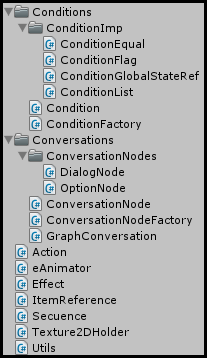
\includegraphics[height=3in]{figures/it1/utilclasses.png}}
	\caption[Clases de Utilidad - Prototipo 1]{Vista de carpeta de las clases de utilidad implementadas en la primera iteración.}
	\label{utilclassesit1}
\end{figure}


La explicación de las clases de utilidad se realiza de forma separada debido a que las clases de utilidad contienen funcionalidad muy diferente entre ellas y no se puede unificar la explicación de las mismas.

\subsection{La clase Texture2DHolder}

La clase Texture2DHolder surge debido a la necesidad de realizar carga de imágenes de manera transparente al usuario, solicitando únicamente al Texture2DHolder que realice la carga de una imagen, a partir de un directorio o unos bytes. Asimismo, esta ayuda a la carga y transformación de imágenes en hilos, ya que Unity3D no permite la carga mediante el método que facilita para carga de recursos, \textit{Resources.Load()}, fuera del bucle principal de ejecución.

Para solventar el problema de la carga paralela de recursos, en lugar de utilizar \textit{Resources.Load()}, se utiliza la librería de sistema, System.IO, utilizando carga de bytes directamente, almacenándolos temporalmente en un \textit{array} de \textit{bytes} dentro de si mismo. para obtener los datos de los ficheros directamente.

Esto causa un pequeño problema a la hora de generar un paquete, y es que, si se desea generar un juego con los recursos incluidos dentro del sistema de empaquetado de Unity, no se podrá acceder a estos recursos, ya que la librería System.IO busca los ficheros en el sistema de ficheros, y \textit{Resources.Load()}, en su lugar, obtiene dichos recursos de los paquetes comprimidos de recursos generados. En la versión final del proyecto, ambos tipos de cargas están permitidos.

Asimismo, Unity no permite generar una \textit{Texture2D}\footnote{Una Texture2D es la clase que se utiliza para guardar texturas bidimensionales en Unity3D, como imágenes, fotografias, o sprites.} si no es en tiempo de ejecución, por lo que, en el momento de la carga sólo se obtienen los bytes, y no es hasta el momento en el que la textura se utiliza por primera vez.

\begin{lstlisting}
public Texture2D LoadTexture(bytes[] fileData)
{
	Texture2D tex = new Texture2D(2, 2,TextureFormat.BGRA32,false);
	tex.LoadImage(fileData);
	return tex;
}
\end{lstlisting}

Tras esto la textura queda guardada y no se vuelve a generar, por lo que se reduce el tiempo de ejecución del programa, a coste de sacrificar memoria. En este caso, como las texturas de los videojuegos generados con eAdventure no ocupan más que el propio juego en sí mismas, se asume que, el coste en memoria de la aplicación no será muy elevado.

\subsection{La interfaz Sequence: Effect, Conversation y Condition})
\label{sequencessecit2}

La interfaz \textit{Sequence} surge de la necesidad de generar una interfaz para interactuar con los efectos y las conversaciones, elementos que son capaces de ejecutarse y realizar tareas que pueden tener alto nivel de complejidad. Esta interfaz, en esencia, provee de un método \textit{public bool execute()}, la cual ejecuta el contenido de si mismas, y devuelve verdadero en caso de que, la secuencia necesite esperar, ya sea por la necesidad de interacción del usuario, o por que un elemento debe ejecutarse un tiempo determinado.

Pese a que la interfaz \textit{Sequence} seguirá existiendo en la versión final del proyecto, se ampliará utilizando la interfaz \textit{Interactuable}, para poder solicitar al usuario que interactúe con algún elemento, ya sea una secuencia, o un elemento interactivo de la escena.

\subsubsection{La clase Effect}

La clase \textit{Effect} es una clase que es híbrida entre Clase de Datos y Clase de Utilidad, pues recibe un \textit{XmlElement} para generarse, y sin embargo aporta funcionalidad por sí misma. Lo que hace dicha clase es: Obtiene un listado de \textit{EffectNode} y de \textit{Condition} y, si existen condiciones, las asigna a cada nodo para que este únicamente se ejecute si cumple las condiciones que permiten su ejecución.

Esta clase contiene dentro de su fichero la clase \textit{EffectNode} el cual, a su vez, contiene cada una de las descripciones de los nodos de una secuencia de efectos. Se implementó en esta iteración del proyecto con una bifurcación, utilizando un \textit{Switch}, en lugar de hacer herencia debido a la cantidad de nodos diferentes, no obstante, en la versión final del proyecto, existen clases para tratar cada uno de los nodos de efecto que componen la secuencia de efectos.

Los \textit{EffectNode} realizan tareas como activar una \textit{Flag}, poner una variable, ejecutar una \textit{Macro}, o ejecutar una condición, por ello tienen dos variables de control que definen su funcionamiento, y una función \textit{execute()} que los pone en funcionamiento. Estas dos variables de control sirven para determinar si dicho nodo sólo se ejecuta una vez, o varias, y para controlar cuántas veces se ha ejecutado ya dicho nodo. Hasta que un nodo no determina que ha completado su ejecución, este no permite que la secuencia se siga ejecutando.

\subsubsection{Las clases GraphConversation y Condition}
\label{linqit1}

Estas clases son las más extensibles de todas las clases que se implementaron en la primera iteración del proyecto. Ambas tienen una factoría para generarse, ya sea \textit{ConditionFactory} y \textit{DialogNodeFactory}, y se generan automáticamente a partir de un \textit{XmlElement}, que contiene la especificación extraída del archivo de especificación del juego.

Por su parte \textit{GraphConversation} solicita a \textit{DialogNodeFactory} un nuevo \textit{DialogNode} por cada uno de sus hijos, y así se genera el diálogo. La “magia” de \textit{DialogNodeFactory} y de \textit{ConditionFactory} es que utilizan \textit{System.Linq}\footnote{El espacio de nombres System.Linq proporciona clases e interfaces que admiten consultas que utilizan Language-integrated query (LINQ)} para examinar el espacio de nombres y obtener de ahí todas las clases que implementan la interfaz \textit{DialogNode} o \textit{Condition}. Esto se realiza de la siguiente manera:
\begin{lstlisting}
types = System.AppDomain.CurrentDomain.GetAssemblies ().SelectMany (s => s.GetTypes ()).Where (p => typeof(ConversationNode).IsAssignableFrom (p)).ToList();

types.Remove(typeof(ConversationNode));
\end{lstlisting}

Y una vez que se ha obtenido la lista de tipos que implementan dicha interfaz, se realiza una búsqueda secuencial, preguntando a cada clase si puede realizar la lectura de dicho \textit{XmlElement}. En caso afirmativo, se le pide que se construya a partir de dicho documento, y la factoría devuelve dicho elemento. Las funciones \textit{canParseType()} y \textit{parse()} están dentro de las inferfaces \textit{DialogNode} y \textit{Condition}. Esto se ve representado en el código que se presenta a continuación:

\begin{lstlisting}
foreach (System.Type t in types)
{
	ConversationNode tmp = (ConversationNode) System.Activator.CreateInstance(t);
	
	if(tmp.canParseType(node.Name))
	{
		tmp.parse(node);
		return tmp;
	}
}
\end{lstlisting}


De esta forma, obtenemos un diseño sencillo y cómodo de extender, pues añadir nuevos tipos de nodo de conversación, o tipos de condiciones es una tarea tan sencilla como generar una nueva clase que implemente esas interfaces, y automáticamente, y sin la necesidad de incluir la existencia de dicha interfaz en la factoría, automáticamente se utiliza.

Si se desea entender o extender el conocimiento de la implementación de estas clases se recomienda mirar el código de estas clases, pues es bastante sencillo y da una visión mucho más clara de su funcionamiento.

\subsection{La clase Action}

Esta clase es tan simple como un efecto con representación. Está compuesta por un Effect que se ejecuta cuando se realiza la acción, una Condition que determina cuando esa acción está disponible, y una serie de recursos que se utilizan para su representación.
La gestión de la visualización de las acciones se realiza en Game, en la funcion OnGUI().

\section{Acerca de los elementos de Adaptación}

El juego Checklist cuenta con un elemento adicional para el jugador, las Adaptation estas no son más que una serie de estados iniciales del juego para que, el juego pueda adaptarse al jugador, ya sea por motivos de accesibilidad o por motivos de nivel.
Las Adaptation se han implementado, pero no existe ningún mecanismo que permite decidir cuál Adaptation se selecciona en cada momento, sino que se selecciona una aleatoriamente al comienzo del juego, y tras esto se trabaja siempre con la misma.

